%!TEX root = main.tex

\section{Numerical solutions}
\label{sec:numerics}
\subsection{Identification of equilibrium branches}

% We now switch to the study of  the nonlinear regime  and we will resort to numerical calculations  to explore the system's behavior beyond the linear approximation.
We now turn our attention to the solutions beyond the trivial homogeneous branch and will use numerical calculations to identify the equilibrium branches corresponding to the inhomogeneous solutions. Our goal is to construct an \emph{equilibrium map} that represents all stable and unstable equilibrium states as a function of the external load~\cite{Pattamatta2014-pn}\comment[id={OUS}]{add reference}
.

To find the equilibrium branches we make use of a pseudo-arclength continuation technique implemented in the software AUTO~\cite{Doedel1981-sa}, \comment[id={OUS}]{add reference} see also \cite{Pattamatta2014-pn}. It solves the nonlinear equations \ref{auto1} and \ref{auto2} in the case of rigid and compliant foundation, respectively, with the end displacement $\bar\epsilon_t$ treated as a continuation parameter. To discretize the boundary-value problem, it uses collocation with Lagrange polynomials, and in our simulations we had $N=300$ mesh points with $N_c = 5$ collocation nodes and activated mesh adaptation. 
\begin{figure}
    \hspace*{-3cm}
% 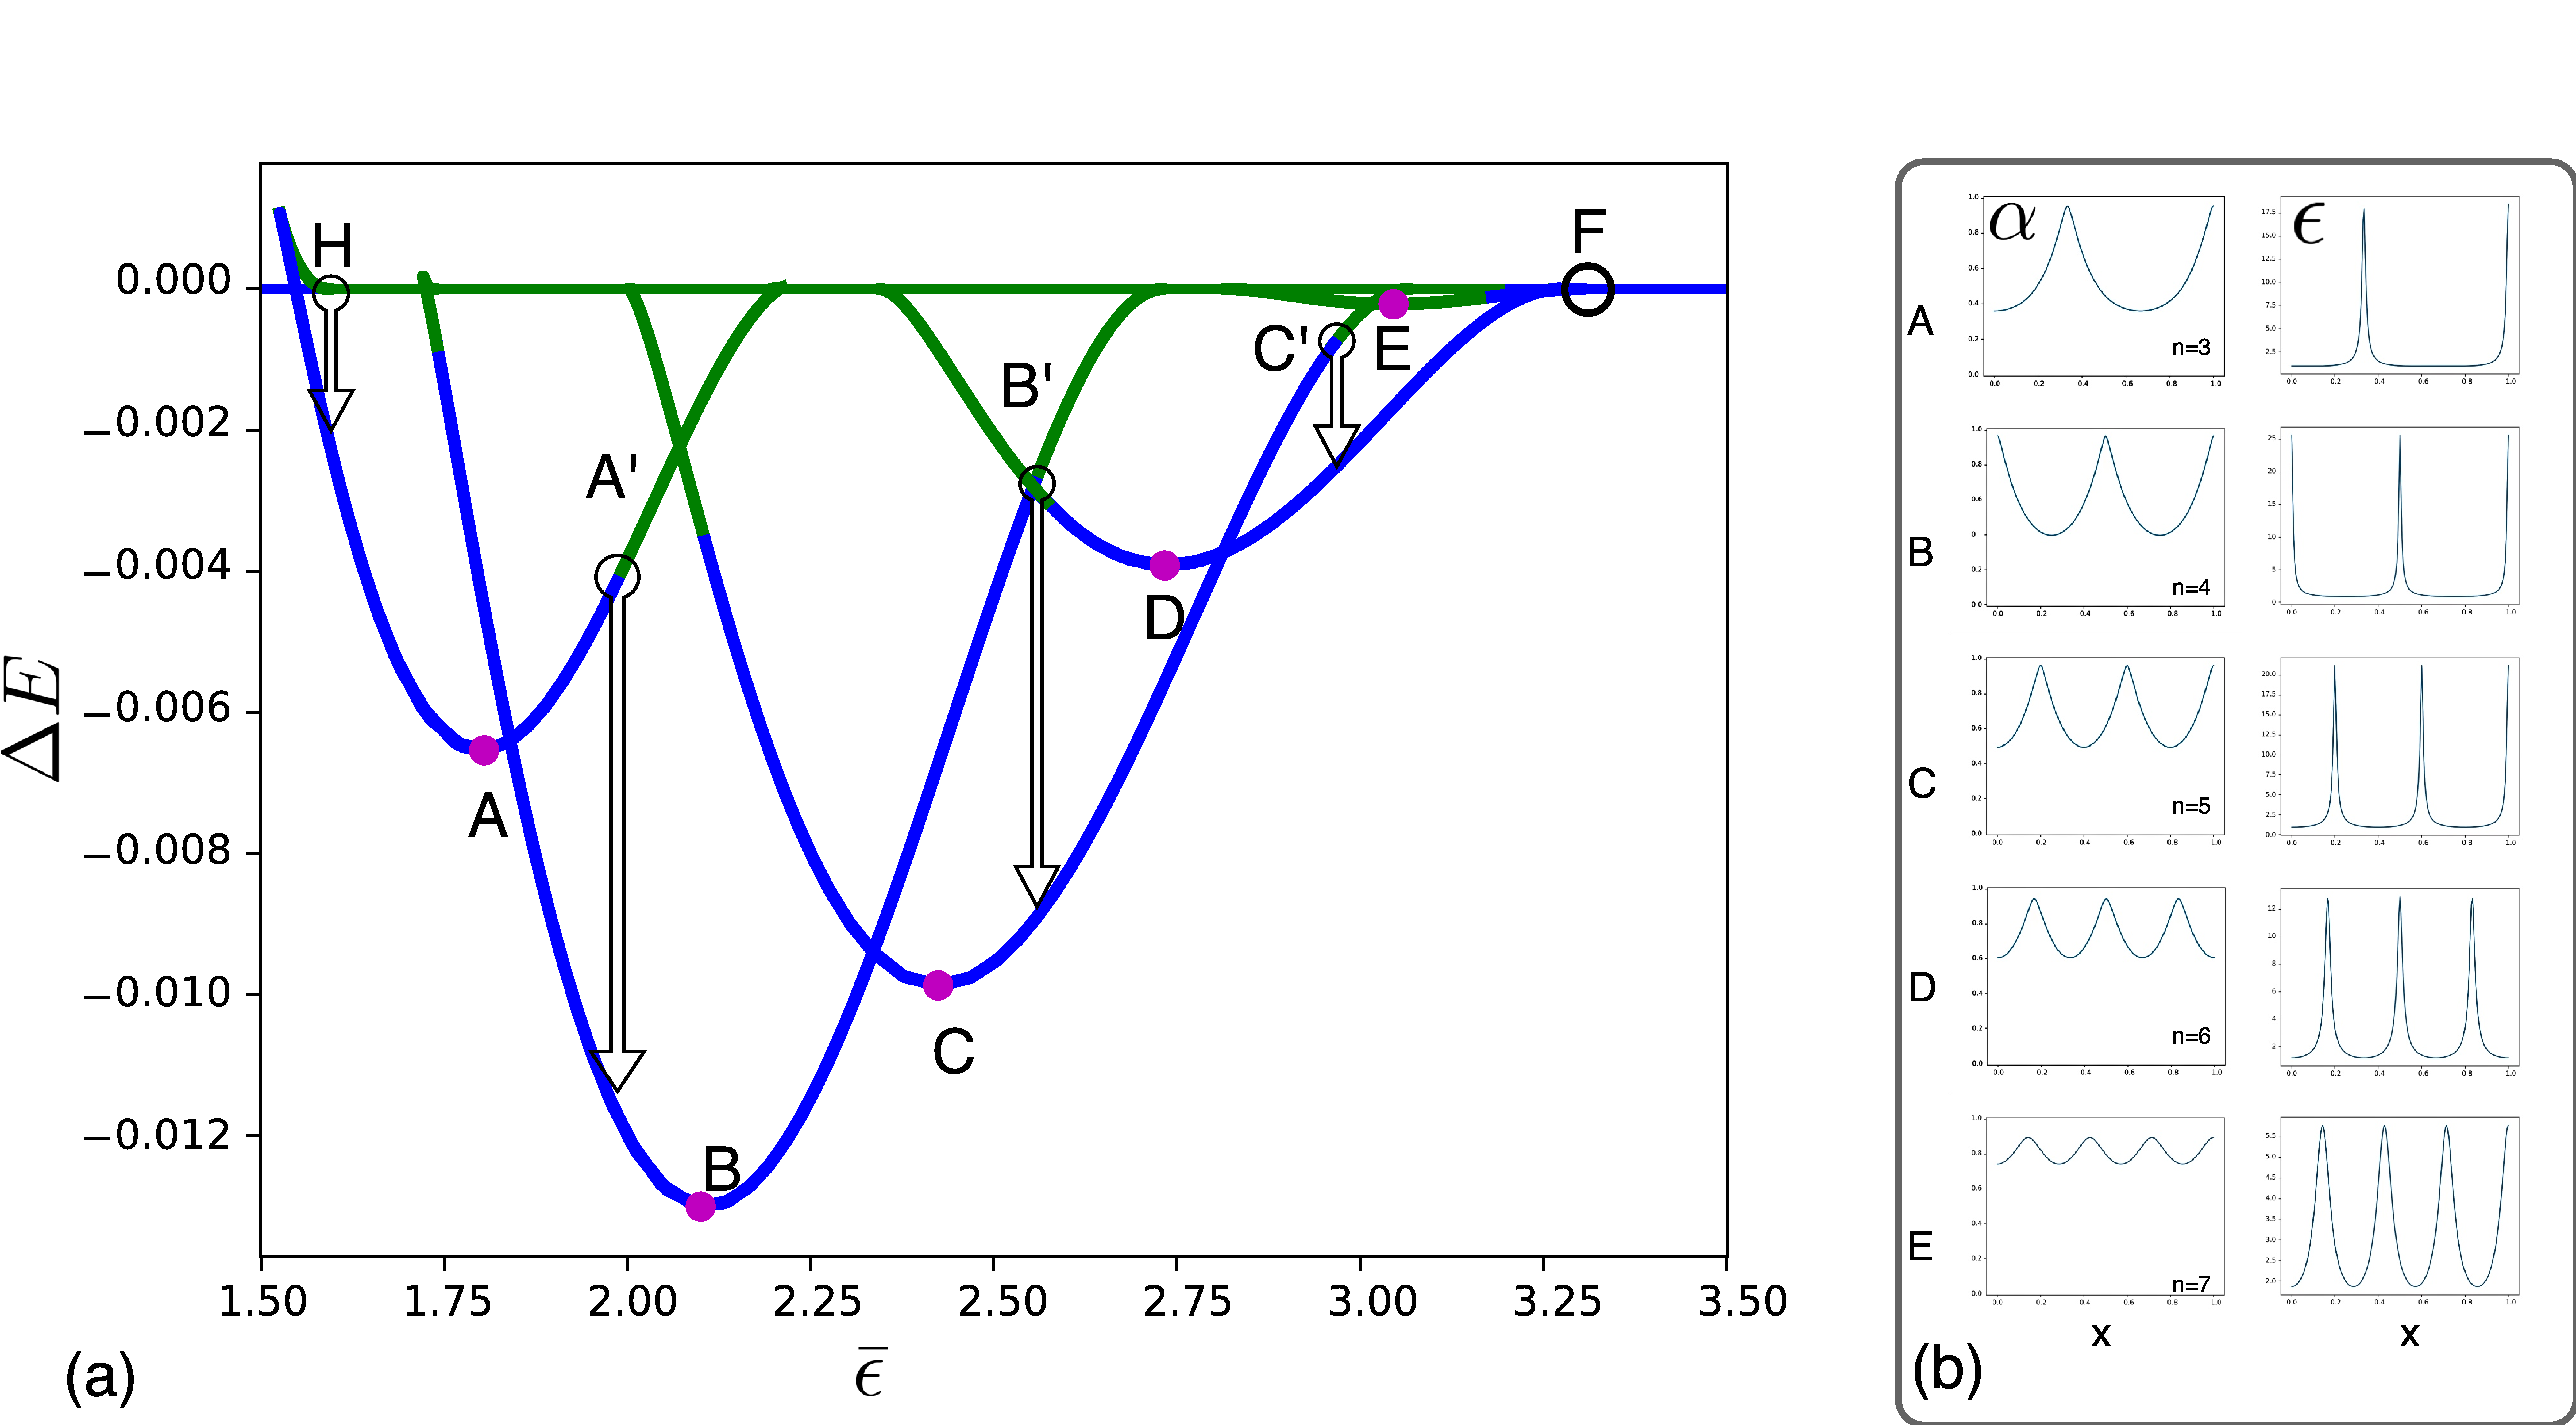
\includegraphics[scale=0.1]{./final_images/fig2.pdf}
\includegraphics[align=c, width=.8\textwidth]{../images/model_stiff_energy.pdf}
\includegraphics[align=c, width=.5\textwidth]{../images/model_stiff_fields.pdf}
    \caption{
% \todo[inline]{Add marker for $\ep_c$ in a), }
Equilibrium branches for phase-field thin film model of an elastic membrane on a compliant elastic foundation. Left, the energy difference $\Delta \Estiff$ between the current and the homogeneous configurations, for the same load. Stability of solutions is color-coded: blue denotes stability while orange indicates instability, by numerical evaluation of the smallest eigenvalue of the stiffness matrix $\stiffmat$. Equilibrium branches are parametrised by an integer $n$ and rrows indicate branch switching events associated with the loss of stability; Right, damage and strain profiles of the minimum energy configurations on each branch.}
    \label{fig:branches-stiff}
\end{figure}
In order to asses the stability of equilibrium branches, we use  the numerical evaluation of the smallest eigenvalue of the second variation by discretizing the integrals \eqref{hessian22} and   \eqref{hessian222} to construct the stiffness matrices
$\stiffmat$ and $\widetilde\stiffmat$, investigating numerically the sign of the minimal eigenvalue $\lambda_t$ of the corresponding discrete quadratic form \cite{Sanderson2016-ht}.  The finite element discretization of the displacement and damage field $(u, \alpha )$     with \( n_u \) displacement degrees-of-freedom 
$
\mathbf{u} = \{ u_1, \ldots, u_{n_u} \}^T 
$
and \( n_\alpha \) damage degrees-of-freedom 
$
\boldsymbol{\alpha} = \{ \alpha_1, \ldots, \alpha_{n_\alpha} \}^T
$ is given by 
$
u(\mathbf{x}) \approx u_{\text{FE}} (\mathbf{x}) := \sum_{i=1}^{n_u} \mathcal{N}^{(u)}_i(\mathbf{x}) u_i $
and $\alpha(\mathbf{x}) \approx \alpha_{\text{FE}} (\mathbf{x}) := \sum_{i=1}^{n_\alpha} \mathcal{N}^{(\alpha)}_i (\mathbf{x}) \alpha_i 
$
where $\mathcal{N}^{(u)}(\mathbf{x}) $ and $\mathcal{N}^{(\alpha)}(\mathbf{x}) $ are the finite element basis functions and  $u_h$ and  $\alpha_h$ are nodal values for the displacement and damage fields, respectively. We used quadratic one-dimensional finite elements with 3 nodes  whose   shape functions   ${\mathcal N}_i(x)$ at a node $i$  are given by ${\mathcal N}_1(\xi)=-0.5\xi(1-\xi)$, ${\mathcal N}_2(\xi)=-0.5\xi(1+\xi)$ and ${\mathcal N}_3(\xi)=-(1-\xi)(1+\xi)$, where $\xi$ is the isoparameteric coordinate. The discrete solution $u(x_i)$ provided at discrete nodes $x_i$ by AUTO was first interpolated using B-spline basis functions of degree 3 \cite{Grimstad2016-cq}, and then utilized to calculate the integrals \eqref{hessian22} and \ref{hessian222} employing a three-point Gauss integration scheme. The fixed boundary conditions were enforced by removing the rows and columns corresponding to $x = 0$ and $x = 1$ from the stiffness matrices 
% $\mathbf{K}^i, i = 1, 2$
$\stiffmat$ and $\widetilde\stiffmat$. The explicit form of the stiffness matrix for the stiff substrate model is given by
\begin{equation}
    \stiffmat = 
    % \stiffmat^1=
    \begin{bmatrix}
\int_0^1[ \frac{1}{\Lambda^2}{\mathcal N}_i{\mathcal N}_j + (1-\alpha)^2{\mathcal N}'_i{\mathcal N}'_j
%+\frac{1}{\Lambda^2}{\mathcal N}_i {\mathcal N}_j
] dx&
-2\int_0^1(1-\alpha)u' {\mathcal N}'_i {\mathcal N}_j  dx\\
-2\int_0^1(1-\alpha)u' {\mathcal N}_i {\mathcal N}'_j dx
& \int_0^1 [ (2+u'^2){\mathcal N}_i{\mathcal N}_j +\damagell^2{\mathcal N}'_i{\mathcal N}'_j] dx
\end{bmatrix},
\label{eq:stifness1}
\end{equation}
whereas the compliant substrate model it reads
\begin{equation}
    \stiffmatcompl=
    % /\stiffmat^2=
    \begin{bmatrix}
    \int_0^1[ \frac{1}{\Lambda^2}{\mathcal N}_i{\mathcal N}_j + (1-\alpha)^2{\mathcal N}'_i{\mathcal N}'_j] dx&
-2\int_0^1(1-\alpha)u' {\mathcal N}'_i {\mathcal N}_j  dx&
-\int_0^1[\frac{1}{\Lambda^2}{\mathcal N}_i {\mathcal N}_j]  dx\\

-2\int_0^1(1-\alpha)u' {\mathcal N}_i {\mathcal N}'_j dx&
 \int_0^1 [ (2+u'^2){\mathcal N}_i{\mathcal N}_j +\damagell^2{\mathcal N}'_i{\mathcal N}'_j] dx&
 0\\

-\int_0^1[\frac{1}{\Lambda^2}{\mathcal N}_i{\mathcal N}_j ] dx
&0
&\int_0^1\frac{1}{\Lambda^2}{\mathcal N}_i {\mathcal N}_j+r_s{\mathcal N}'_i {\mathcal N}'_j  dx
\end{bmatrix}.
\label{eq:stifness2}
\end{equation}
Our objective is to establish a branch switching strategy that,
as the external loading parameter monotonically increases, allows equilibrium branch transitions when the current branch ceases to be stable or to exist.
% as part of our model's energetic definition. 
This strategy must ensure the system's re-stabilization following an instability in a dissipative manner. In a quasi-static scenario, it should select a new locally stable equilibrium branch with inherently lower energy.  Considering applications in structural mechanics, our approach to selecting the new equilibrium branch relies on a criterion of local energy minimization (LEM) which emulates the zero viscosity limit of overdamped viscous dynamics. This approach differs from a global energy minimizing (GEM) strategy, which may be more relevant in biomechanical applications~\cite{Salman2021-mn}. According to LEM protocol, during quasi-static loading, the system will remain in a metastable state (a local minimum of energy) until it becomes unstable. Subsequently, during an isolated switching event, the new equilibrium branch will be chosen using a descent algorithm \cite{Puglisi2005-lg}.
\begin{figure}
    %\centering
    \hspace*{-3cm}
% 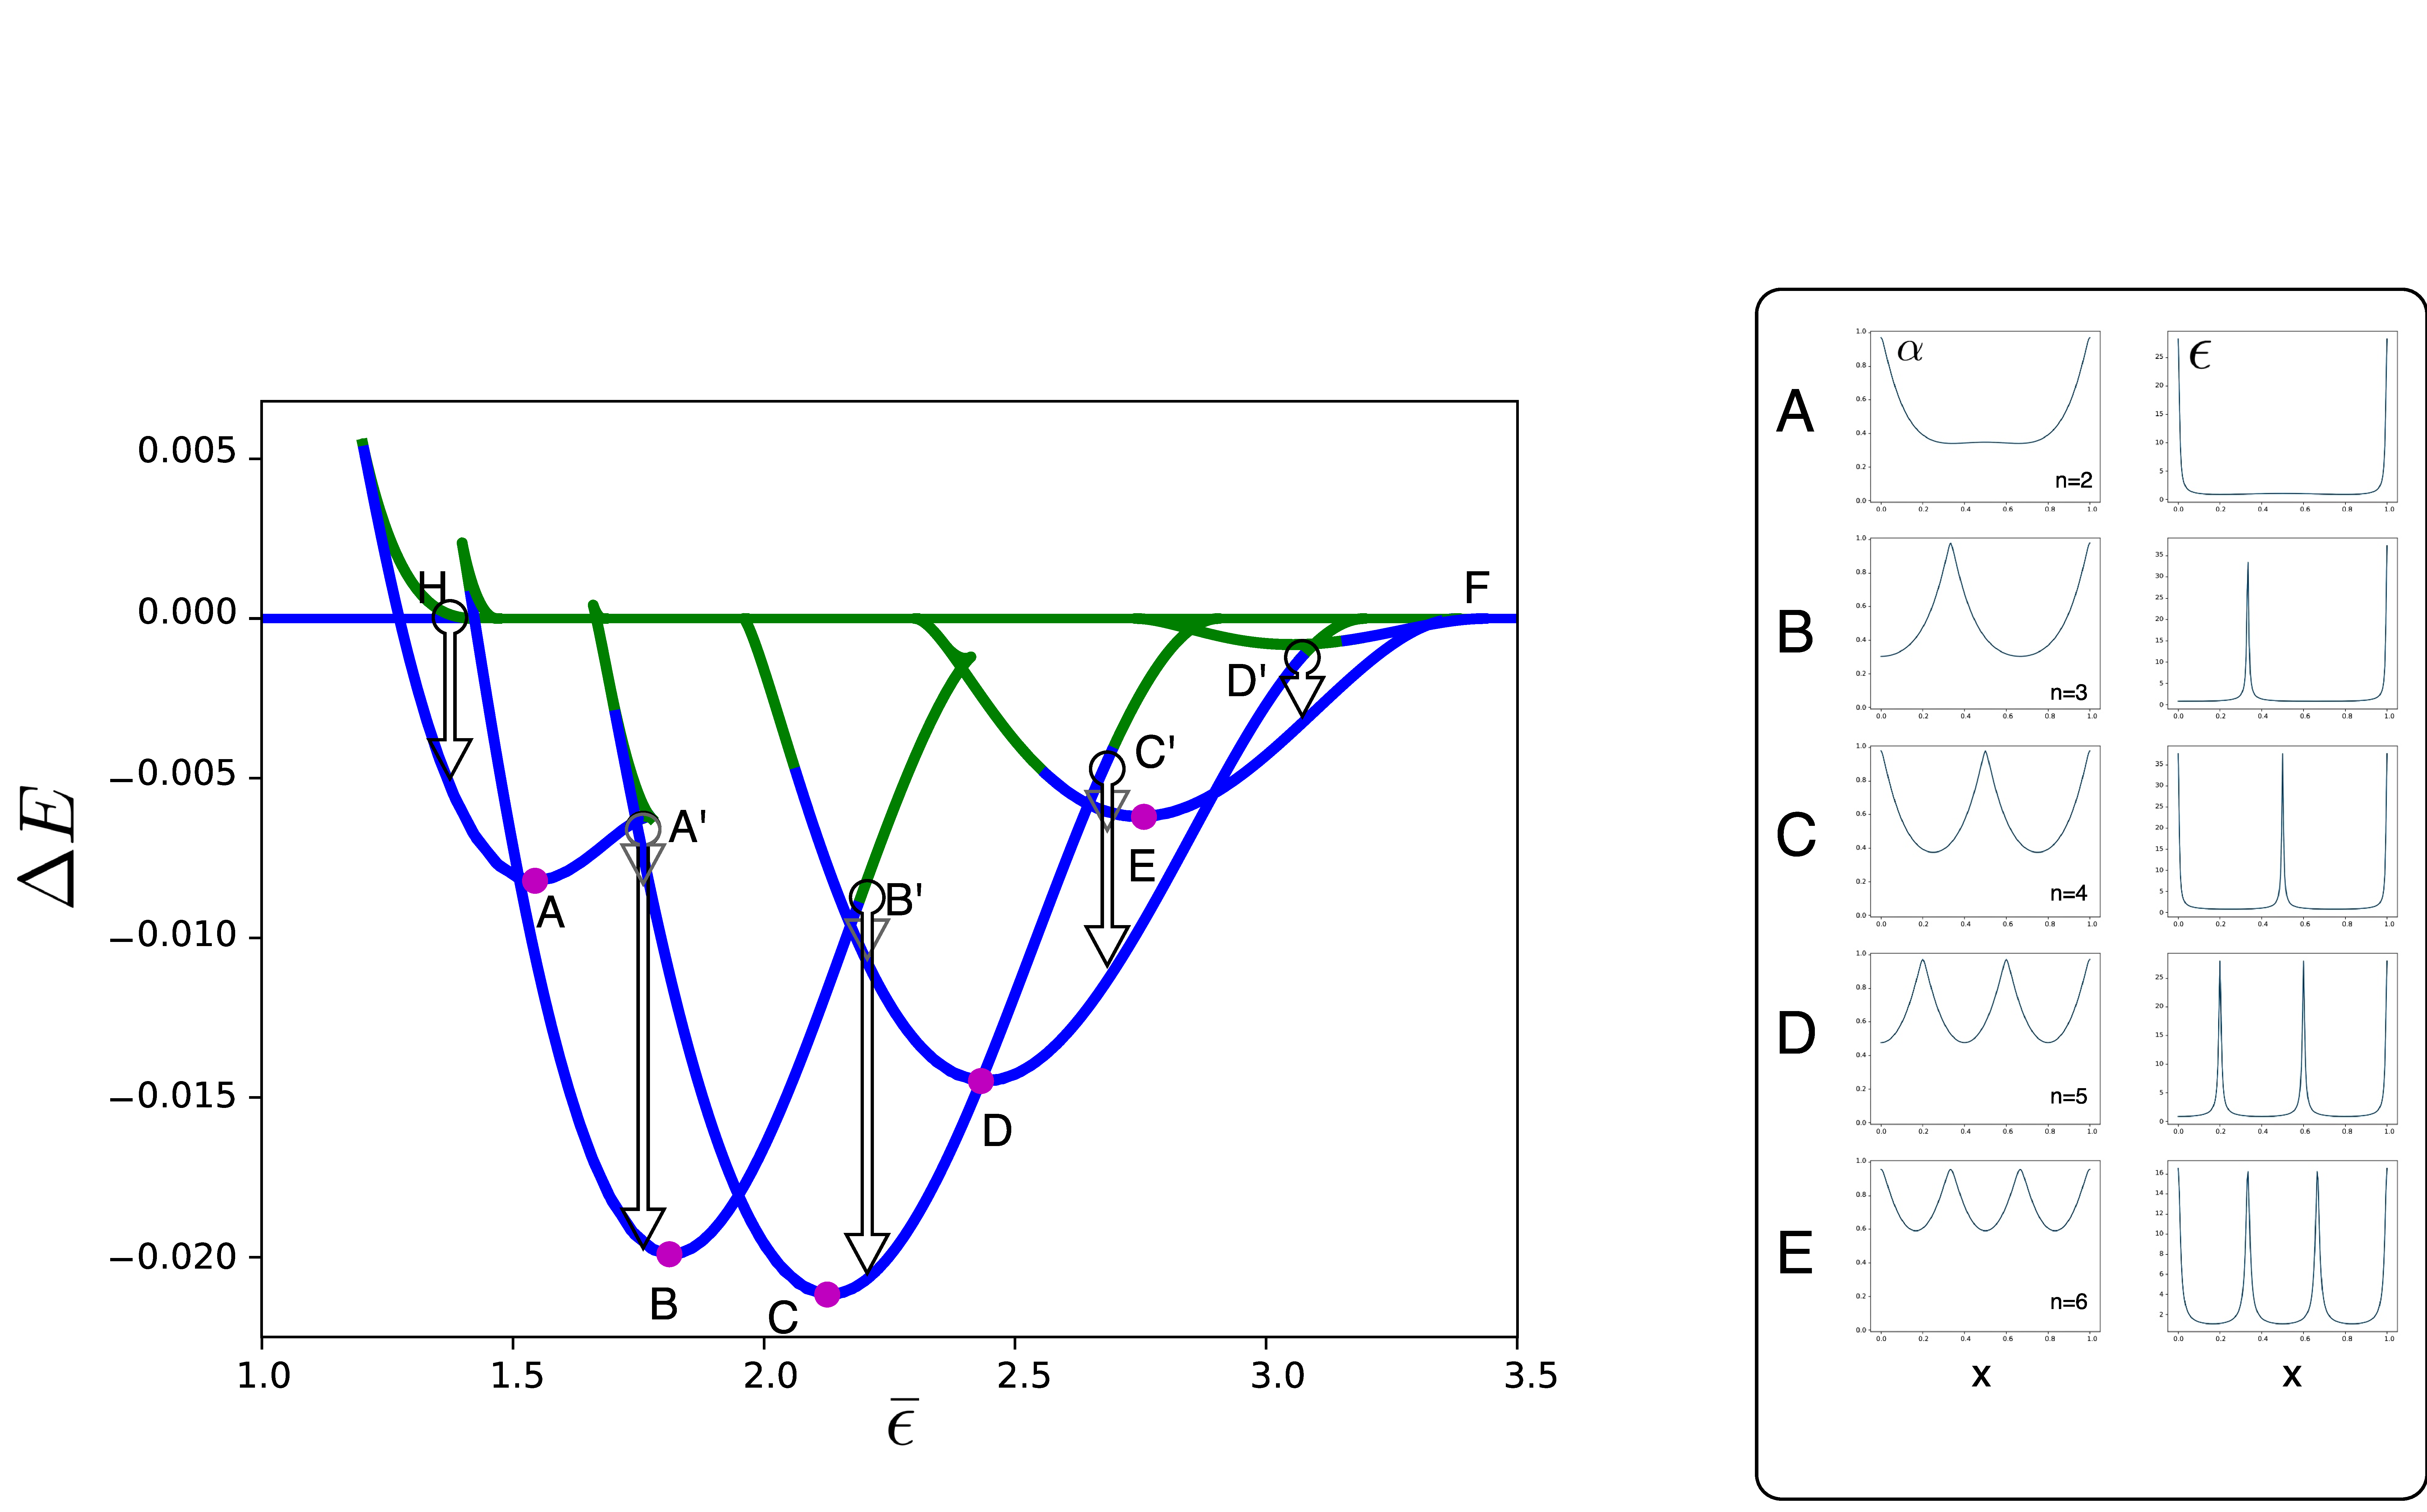
\includegraphics[scale=0.1]{./final_images/fig3.pdf}
\includegraphics[align=c,width=.8\textwidth]{../images/model_compliant_energy.pdf}
\includegraphics[align=c,width=.5\textwidth]{../images/model_compliant_fields.pdf}
\caption{
% \todo[inline]{
%     Add marker for $\ep_c, H$ in Fig (a)
%     Add marker for $n=1, 2, ...$ in Fig (a)
%     }
Equilibrium branches for phase-field thin film model of an elastic membrane on a compliant elastic foundation. Left, the energy difference $\Delta \Ecompl$ between the current and the homogeneous configurations, for the same load. Stability of solutions is color-coded: blue denotes stability while orange indicates instability, by numerical evaluation of the smallest eigenvalue of the stiffness matrix $\stiffmatcompl$. Equilibrium branches are parametrised by an integer $n$; Right, damage and strain profiles of the minimum energy configurations on each branch.}
    \label{fig:branches-compliant}
\end{figure}

We display the equilibrium branches that solve the nonlinear equations~\ref{auto1} in Fig. \ref{fig:branches-stiff}. These branches are represented in Figure~\ref{fig:branches-compliant} by plotting the energy difference $\Delta \Psi$ between the energy of the current solution and the energy of the homogeneous solution $\Psi_h(\bar{\epsilon_t})$ at the current value of the loading parameter $\bar\epsilon_t$. The stability of solutions is color-coded, light blue and orange representing stable and unstable solutions, respectively. Stability is discerned through numerical evaluation of the smallest eigenvalue $\lambda_t$ of the stiffness matrix $\stiffmat$ (and $\stiffmatcompl$) defined in \eqref{eq:stifness1} (respectively, in \eqref{eq:stifness2}). Eigenvalues represent the local curvatures of the energy functional, so the sign of the smallest  $\lambda_t$ determines the stability of the solution, with $\lambda_t > 0$ indicating stability and $\lambda_t < 0$ indicating instability.

Under the LEM protocol, the system explores the fundamental branch where the homogeneous solution is stable until  \comment[id={OUS}]{we defined $\bar\epsilon^*$ before }
$\bar\epsilon_1=\bar\epsilon^*$, identified using linear stability analysis, see Figure~\ref{fig:branches-stiff}. At the critical load on the homogeneous branch  at point $H$, a first instability determines a branch switching transition, from the trivial branch with $n = 0$ to the nontrivial equilibrium branch with $n = 3$. The ensuing non-homogeneous configuration is linearly stable, as seen in Fig. \ref{fig:branches-stiff}. We depict the lowest energy configuration on this equilibrium branch in Fig.~\ref{fig:branches-stiff} at point $A$, consisting of two simultaneously nucleated localized cracks, one inside the domain and one on the boundary. 

When the loading parameter $\bar{\epsilon}_t$ is further increased, the equilibrium configuration with $n=3$ loses linear stability at point $A'$. In Fig. \ref{fig:branches-stiff} we represent state transitions according to the LEM protocol by arrows. It can be observed that under this protocol, the only available transition from point $A'$ is to the branch with $n=4$, which is locally stable within at the corresponding applied strain $\bar{\epsilon}_2$. The minimum energy configuration on the branch with $n=4$ is depicted in Fig.~\ref{fig:branches-stiff}-right at point $B$, consisting of two cracks: one inside the domain and two on the right and left boundaries.

Further increasing the load, the stability of the branch with $n=4$ is lost at point $B'$, a single available transition leads the system to the branch with $n=5$. While the branch with $n=6$ appears accessible due to its lower energy compared to the current state, it is unstable at the current value of $\bar\epsilon_3$. The lowest energy configurations on the branches with $n=5$ and $n=6$ are illustrated in Fig.~\ref{fig:branches-stiff}-(X-X). Increasing the load along the branch with $n=5$ which loses linear stability at point $C'$, a branch switching event occurs towards the branch with $n=7$, the corresponding minimum energy configuration on this branch is depicted in Fig.~\ref{fig:branches-stiff}(b). Finally, this branch reconnects to the homogeneous branch with $n=0$ at point $F$. Remark that, in the case of a stiff substrate, the LEM protocol identifies a unique evolution path, with the system having a single bifurcation option, or available branch, at each instability point.

For the compliant substrate model, the equilibrium branches that solve the nonlinear equations (Eq.~\ref{auto2}) are shown in Fig.~\ref{fig:branches-compliant}. 
We again plot the energy difference $\Delta \widetilde\Psi$ between the energy of the current solution and the energy of the homogeneous solution $\Estiffhom (\bar{\epsilon})$ at the current value of the loading parameter $\bar\epsilon$. 
The stability of solutions is color coded (light blue indicates \emph{stable} states, orange identifies \emph{unstable} states), the stability marker being given by the numerical evaluation of the smallest eigenvalue of the stiffness matrix $\stiffmatcompl$, defined in \eqref{eq:stifness2}.

According to the LEM protocol with a loading history starting in the unloaded and sound configuration, the initial transition from the trivial solution to the only available branch with $n=2$ occurs at $\bar \epsilon_1$, marked as point $H$. As illustrated in Fig. \ref{fig:branches-compliant}(b), the damage and strain profiles of the lowest energy configuration at point $A$ is characterised by two boundary cracks. As the loading increases, the system persists on the $n=2$ branch until point $A'$ which marks an instability. The system can now access two equilibrium branches: $n=3$ and $n=4$ shown in gray and black arrows. Fig. \ref{fig:branches-compliant}(b) shows the typical damage and strain profiles on these branches. Branches $n=3$ and $n=4$ feature one bulk crack plus one boundary crack, and one bulk crack plus two boundary cracks, respectively. 

The choice of the subsequent branch transition at point $A'$ will dictate the ensuing crack growth. On branches with $n=3$ and $n=4$, at the instability points $B'$ and $C'$, the system will once again encounter two available equilibrium branches. From $n=3$ branch  at point $B'$, the system can transition to either the $n=4$ or $n=5$ branch. Opting for the $n=4$ branch, the subsequent branch selection occurs at point $C'$, offering branches with $n=6$ or $n=5$. Notably, the $n=5$ branch smoothly reconnects with the trivial solution at point $F$. However, the $n=6$ branch experiences another instability at point $D'$ before rejoining the trivial solution. 

The overall behavior of the compliant substrate model reveals additional complexit, for the current choice of material parameters with more branch switching events and non-uniqueness of the overall response. In the stiff substrate model, the LEM strategy identifies a unique evolution path, while in the compliant substrate model the system can follow eight different trajectories in phase-space, given by the various available path-bifurcation choices. This additional richness provides a good case to test numerical optimization methods, which we will discuss in the following.

\subsection{Equilibrium branch selection in overdamped viscous dynamic}
We consider now the equilibrium solutions reachable through the line-search based quasi-Newton algorithms such as  conjugate gradient or the BFGS optimization, which effectively  mimic the zero viscosity limit of overdamped viscous dynamics~\cite{SALMAN2012219}. Quasi-Newton methods serve as alternatives to Newton's method for locating roots or local extrema of functions. Particularly advantageous in scenarios where computing the Hessian at each iteration is impractical or computationally expensive, these methods circumvent the need for explicit computation of energy derivatives. Instead, they rely on evaluating the function value and its gradient and updating the Hessian by analyzing successive gradient vectors.

Quasi-Newton methods are highly suitable for solving the phase-field equation of fracture, particularly when compared to standard Newton method-based monolithic solvers. Such solvers, which simultaneously  solve the equations for both damage and displacement variables, often falter when confronted with nonconvex energy functionals. For example, as demonstrated in \cite{Wick2017-bo}, the Newton method-based monolithic algorithm does not consistently handle brittle fracture scenarios involving abrupt crack propagation. Recently, quasi-Newton methods, particularly the BFGS variant, have been employed to effectively solve the system of coupled governing equations in a monolithic fashion within the phase-field method of fracture. These methods have demonstrated success in various engineering applications, as evidenced by \cite{Kristensen2020-zy,Wu2020-qk,Salman2021-mn,Liu2022-ix}.

In  this study, it is worth to note that our primary objective is not to provide a comprehensive assessment of quasi-Newton methods on a global scale. Instead, our focus lies in scrutinizing their behavior and performance specifically concerning equilibrium branch selections within our simplified framework, where all branches are readily identified. By narrowing our scope to this specific aspect, we aim to gain insights into the effectiveness and reliability of quasi-Newton methods in reaching stable states of our system.
\begin{figure}
    %\centering
    \hspace*{-3cm}
% 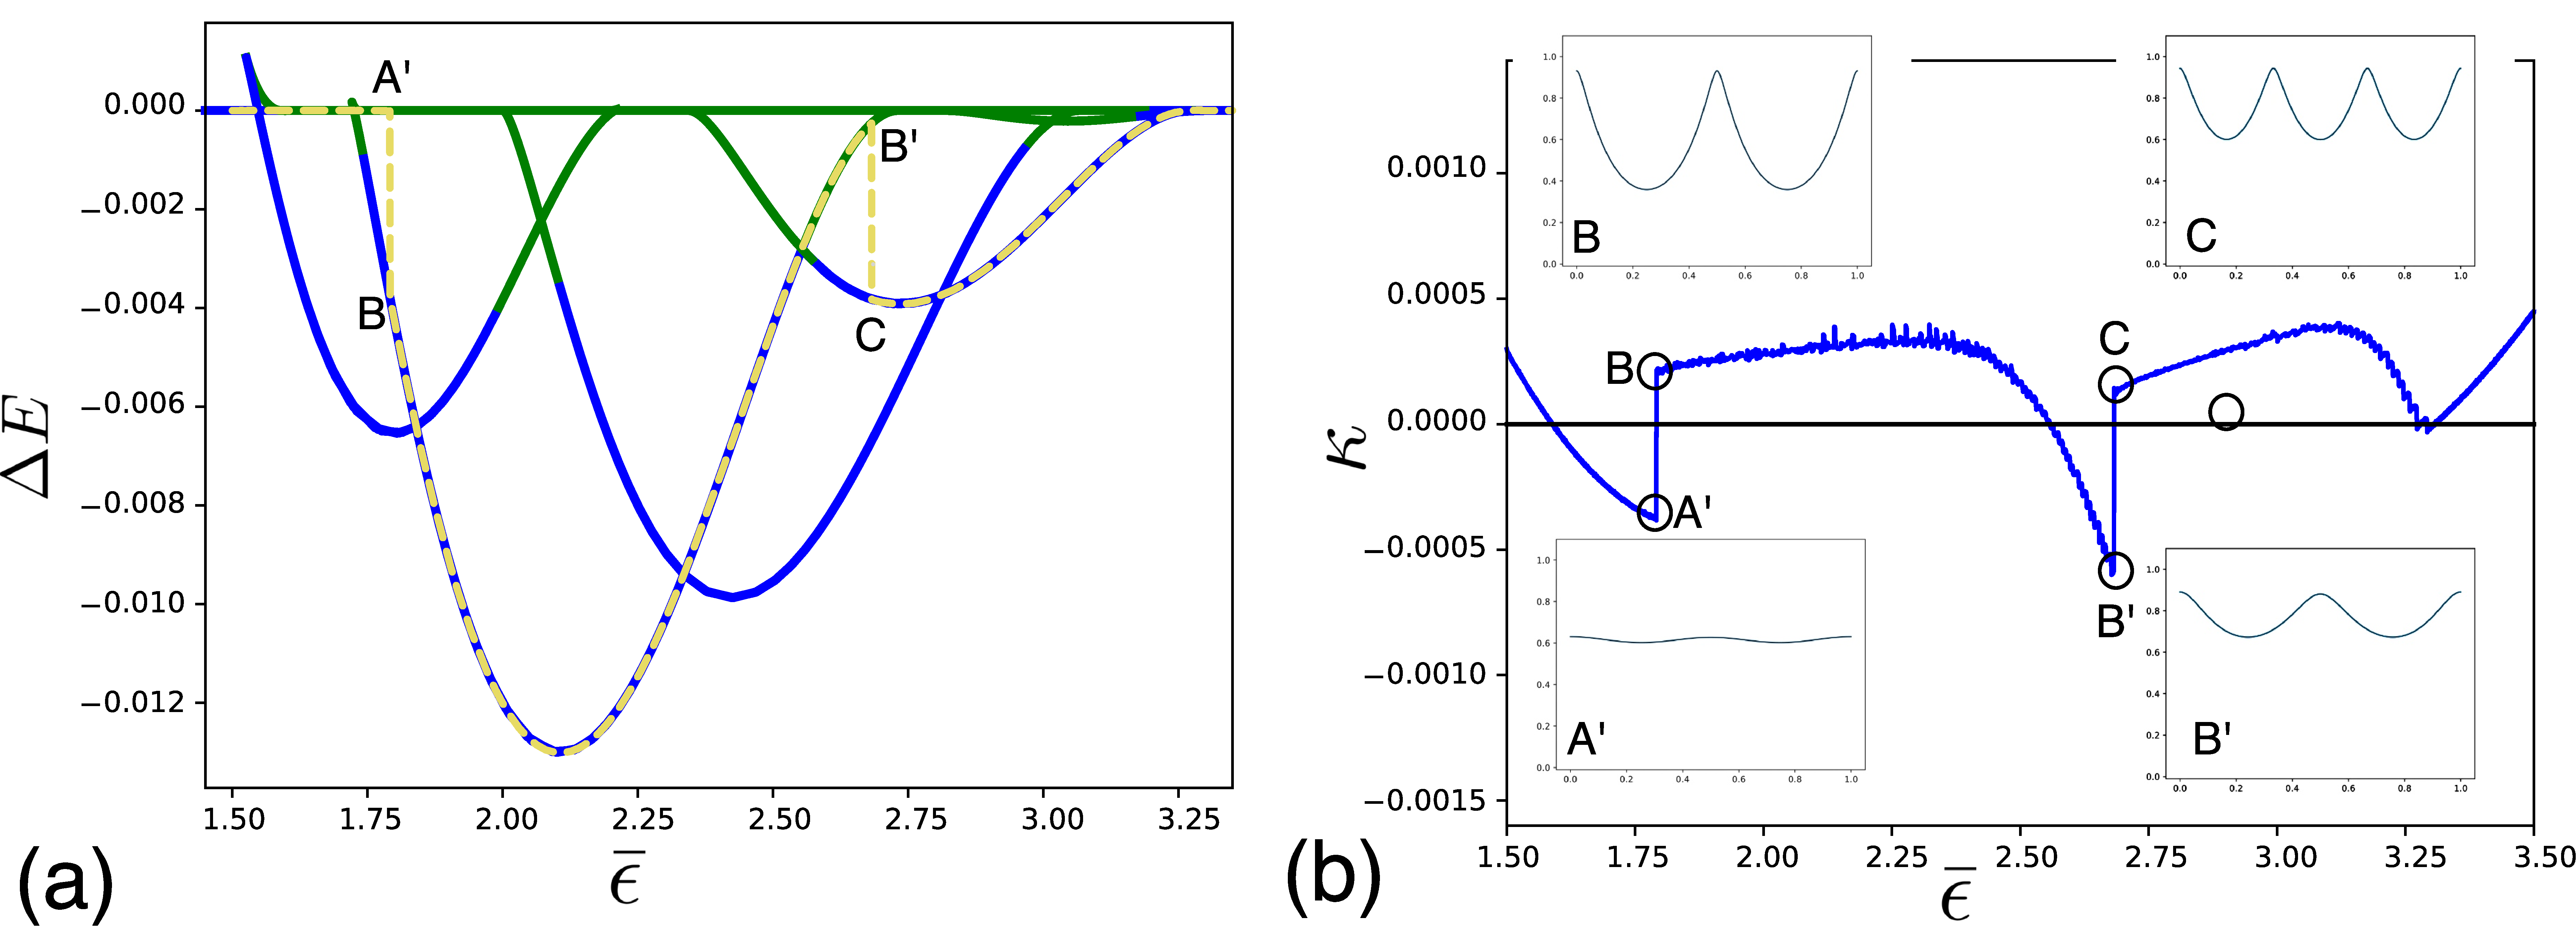
\includegraphics[scale=0.13]{./final_images/fig4.pdf}
\includegraphics[width=.7\textwidth]{../images/model_stiff_energy_kick.pdf}
\includegraphics[width=.4\textwidth]{../images/model_stiff_profiles.pdf}
    \caption{
% \todo[inline]{Add marker for $\ep_c, H$ in Fig (a) and (b)}
Stiff substrate. Quasi-static loading simulations with L-BFGS: (a) the energy difference $\Delta \Estiff$, between the quasi-Newton solutions and the homogeneous solutions are superimposed onto equilibrium branches (light blue: stable; orange: unstable). Bottom, the smallest eigenvalue $\lambda_t$ of the second variation $\Estiff''$ as a function of the loading parameter $\bar\epsilon$. In red, indicated the unstable region $\lambda_t<0$, where the equilibrium solution returned by the solver does not satisfy the evolution law; Right, damage profiles referring to the transition endstates.}
    \label{fig:tempo1}
\end{figure}

Recall that quasi-Newton algorithms only evaluate the function value and its gradient to reach equilibrium configurations. This implies that in our case, we need to evaluate integrals \eqref{def:energy_stiff} and \eqref{def:energy_compliant}, along with their first variations given by \eqref{firstvar1} and \eqref{firstvar}, in the stiff and compliant models, respectively. We   discretized the integrals \eqref{firstvar1} and \eqref{firstvar} to construct the residuals vectors using finite elements to obtain 
\begin{equation}
    {\bf R} =
    %  {\bf R}^1=
     \int_0^1 [(1-\alpha)^2u'\mathcal{N}'_i+\frac{1}{\Lambda^2} (u-\subsu) \mathcal{N}_i+\frac{1}{2}(u'^2 \soften'(\alpha)+\homogdiss'(\alpha))\mathcal{N}_i+\damagell^2\alpha'\mathcal{N}'_i ]dx,\label{residual1}
\end{equation}
in the stiff model and 
\begin{equation}
    \widetilde{{\bf R}}= 
    % {\bf R}^2=
    \int_0^1 [(1-\alpha)^2u'\mathcal{N}'_i+\frac{1}{\Lambda^2} (u-\subsu) \mathcal{N}_i+\frac{1}{2}(u'^2 \soften'(\alpha)+\homogdiss'(\alpha))\mathcal{N}_i+\damagell^2\alpha'\mathcal{N}'_i +
    \rho \subsu'\mathcal{N}_i]dx\label{residual2}.
\end{equation}
in the compliant substrate model. 

Among iterative methods for large-scale unconstrained optimization, particularly when dealing with possibly dense Hessian matrices,  quasi-Newton methods often emerge as preferable alternatives to the widely-used Newton-Raphson (NR) algorithm. The NR algorithm, conventionally utilized for solving linear equations to determine the correction $\Delta \mathbf{X}^{(k)}$ from the current estimate $\mathbf{X}^{(k)} = (\mathbf{u}^{(k)}, \boldsymbol{\alpha}^{(k)})$ at iteration $k$, is expressed in our context as:
\begin{equation}
K_{ij} \Delta X_j^{(k)} + R_i = 0,
\label{Eq:NR}
\end{equation}
where the discrete stiffness matrix $\mathbf{K}$ and bulk forces $\mathbf{R}$ are computed with the initial guess $\mathbf{X}^{(k)}$. Subsequently, the guess is updated as $\mathbf{X}^{(k+1)} = \mathbf{X}^{(k)} + \Delta \mathbf{X}^{(k)}$ after solving Equation \eqref{Eq:NR} using LU factorization~\cite{Sanderson2016-ht}. It's evident that the NR algorithm fails if the discrete stiffness matrix $\mathbf{K}$ isn't invertible.

On the other hand, quasi-Newton methods are well-established (see standard textbooks, e.g., \cite{Nocedal1999-zr,Nocedal2006-qh}), and generate a sequence $\left\{\mathbf{X}^{(k)}\right\}$ according to the following scheme:
\begin{equation}
\mathbf{X}^{(k+1)} = \mathbf{X}^{(k)} + h^{(k)} \mathbf{p} ^{(k)}, \quad k=0,1,\ldots
\end{equation}
with
\begin{equation}
\mathbf{p}^{(k)}=-(\mathbf{B}^{(k)})^{-1}{\bf R},
\end{equation}
where $(\mathbf{B}^{(k)})^{-1}$ approximates the inverse of the Hessian matrix  $\mathbf{K}$ and $h^{(k)}$ represents a step length. Particularly, instead of computing $(\mathbf{B}^{(k)})^{-1}$  at each iteration $k$, these methods update $(\mathbf{B}^{(k)})^{-1}$ in a straightforward manner to obtain the new approximation $(\mathbf{B}^{(k+1)})^{-1}$  for the subsequent iteration. Additionally, rather than storing full dense $N \times N$ approximations, they only retain a few vectors of length $N=n_\alpha + n_u$, enabling implicit representation of the approximations. Moreover, the choice of the step length $h^{(k)}$ is carried out through a line search to minimize a function $f(h) = f(\mathbf{X}^{(k)} + h \mathbf{p}^{(k)})$ in order to find an acceptable step size $h^{(k)}$ such that $h^{(k)} \in \arg \min_{h} f$.

Among quasi-Newton schemes, the L-BFGS method is widely regarded as one of the most efficient and well-suited for large-scale problems due to its limited and user-controlled storage requirements. This method relies on constructing an approximation of the inverse Hessian matrix, leveraging curvature information solely from recent iterations. Note also that the update formula for the approximative in successive minimization steps depends on the adapted algorithm. These algorithms are extensively used in the literature, and we refer the reader to the references for a more detailed description~\cite{Matthies1979-gl,Xu2001-ax,Nocedal1999-zr,Nocedal2006-qh,Simone2012-tx,Lewis2013-eu,Curtis2015-wp}. However, quasi-Newton methods do present certain drawbacks, notably slow convergence for ill-conditioned problems, particularly when the eigenvalues of the Hessian matrix are widely dispersed~\cite{Simone2012-tx}.
\begin{figure}
    \centering
    \hspace*{-2cm}
    \includegraphics[width=.7\textwidth]{../images/model_compliant_energy_kick.pdf}
    \includegraphics[width=.4\textwidth]{../images/model_compliant_profiles.pdf}
    \caption{
        Compliant substrate. Quasi-static loading simulations with L-BFGS: (a) the energy difference $\Delta E$, between the quasi-Newton solutions and the homogeneous solutions are superimposed onto equilibrium branches (light blue: stable; orange: unstable). Bottom, the smallest eigenvalue $\lambda_t$ of the second variation $\Ecompl''$ as a function of the loading parameter $\bar\epsilon$. In red, indicated the unstable region $\lambda_t<0$ for the equilibrium solution; Right, damage profiles referring to the transition endstates.}
    \label{fig:tempo2}
\end{figure}


In our numerical experiments, we employ the BFGS and L-BFGS solvers from the Python SciPy library~\cite{2020SciPy-NMeth} and the Alglib library~\cite{Bochkanov2013-lk}. These solvers utilize the residual vectors (see \ref{residual1} and \ref{residual2}) at each finite element node, alongside the values of integrals \eqref{def:energy_stiff} and \eqref{def:energy_compliant}.
The following results were obtained using the Alglib library~\cite{Bochkanov2013-lk}; however, our findings remain consistent across the other libraries mentioned.



\begin{figure}[htbp]
    \centering
    \includegraphics*[align=c,width=.45\textwidth]{../images/model_stiff_kick_profiles.png}
    \includegraphics*[align=c,width=.45\textwidth]{../images/model_compliant_kick_profiles.png}
    \caption{
        Profiles of damage fields and perturbations showing the effect of the kick algorithm in state transitions (from unstable to stable). Branch switching events correspond to load values indicated by $\bar \epsilon_i$ with $i\in \mathbb N$ in \textcolor{blue}{Fig.~\ref{fig:tempo1} and ~\ref{fig:tempo2}}. The stiff substrate model is in the left column, the compliant substrate model on the right and  the light (orange) line indicates the unstable damage field $\alpha^*$, the eigenvector associated to the smallest eigenvalue, $p$, is displayed in green highlighting its positive and negative values. The dashed line represents the perturbed damage field  $\alpha^*+p$ used as initial guess for the state transition, the solid black line displays the solution $\alpha_t$ returned after first-order convergence.}
    \label{fig:kick}
\end{figure}



% \begin{figure}
%     %\centering
% \includegraphics[width=\textwidth]{./final_images/fig6.pdf}
%     \caption{
% % \todo[inline]{Fix legend colours in (a)}
% Kick algorithm for the first model: (first column) the current unstable solution  for the damage field \added[id=ALB]{(blue)}, the \added[id=ALB]{eigenvector associated to the} smallest \replaced[id=ALB]{eigenvalue}{eigenvector} of this state \added[id=ALB]{(orange)}, and the perturbed damage field with this eigenvector \added[id=ALB]{(green)}; (second column)  the solution returned by the quasi-Newton algorithm wherein initial guess is taken to be the perturbed damage field.
%  }
    
%     \label{fig:kick}
% \end{figure}


% \begin{figure}
%     %\centering
% % \includegraphics[width=\textwidth]{./final_images/fig7.pdf}
%     \caption{Kick algorithm for the second model: (first column) the current unstable solution  for the damage field, the smallest eigenvector of this state, and the perturbed damage field with this eigenvector; (second column)  the solution returned by the quasi-Newton algorithm wherein initial guess is taken to be the perturbed damage field.
%  }
%  \label{fig:kick2}
% \end{figure}

%To summarize, we initially provide the algorithms with an initial guess for $\mathbf{X}^{(k)} = (\mathbf{u}^{(k)}, \alpha^{(k)})$ at a fixed value of the loading parameter $\bar\epsilon$. Additionally, we specify an initial guess for the Hessian matrix, denoted as $\mathbf{B}^{k} \in \mathbb{R}^{n \times n}$. This matrix can either be set as the identity matrix or the uncoupled stiffness matrix to ensure a symmetric and positive definite approximation. Subsequently, the quasi-Newton algorithm computes a search direction using  the analogue of the Newton equation $\mathbf{B}^{(k)} \mathbf{p}^{(k)}  = -\mathbf{R}^{(k)} $,where $\mathbf{p}^{(k)}$ denotes the search direction at stage $k$. Afterwards, it  performs a line search to minimize a function $f(h^{(k)}) = f(\mathbf{X}^{(k)} + h^{(k)} \mathbf{p}^{(k)})$ in order to find an acceptable step size $h^{(k)}$ such that $h^{(k)} \in \arg \min_{h} f$. The solution is then updated in the direction of $\mathbf{p}^{(k)}$ with the step size $h^{(k)}$. 


In Figure \ref{fig:tempo1}, we present the results of our numerical experiments, overlaying solutions obtained with the quasi-Newton algorithm onto the equilibrium map determined using the pseudo-arclength continuation method described in the previous section. Fig. \ref{fig:tempo1}-bottom shows the smallest eigenvalue $\lambda_t$ whose positivity informs on the stability of the solution. All the branch switching events are delayed in the sense they do not take place when the smallest eigenvalue of the second variation vanishes but only beyond the loads corresponding to the eigenvalue's sign transition. Notably, the expected first branch switching event—from the {homogeneous} solution to the branch with \(n=3\) as outlined in the LEM protocol—did not occur at point $H$ as anticipated. During a monotonic loading, the system remains on the trivial branch, as shown in Fig. \ref{fig:branches-stiff}(a), until it transitions to the branch with \(n=4\) at a value of the load much higher than the critical loading parameter \(\bar{\epsilon}_1\). By monitoring the smallest eigenvalue of the second energy variation at the solution, we observe that indeed the solutions computed via the quasi-Newton solver are unstable beyond \(\bar{\epsilon}_1\), which is consistent with the linear stability results for the trivial branch. A closer inspection of the solution field reveals that the quasi-Newton solutions are not homogeneous but instead exhibit a small perturbation akin to the instability mode calculated analytically (i.e., the eigenvector associated with the smallest eigenvalue). For instance, the  quasi-Newton solution before the first branch switching event is shown in inset (state $H$) in Fig. \ref{fig:tempo1}-right, where we see that the equilibrium damage shows a slight oscillation reminiscent of the eigenmode \(\alpha_n(x) \sim \cos(n\pi x)\), with \(n=3\). The state transition captured by the quasi-Newton method is the one towards the \(n=4\) branch, with one bulk crack and two boundary cracks, see inset (X) in Fig. \ref{fig:tempo1}-right. If the transition had taken place at \(\bar{\epsilon}_1\) as anticipated by our LEM strategy, the system would have reached a configuration with two bulk cracks and one boundary crack, as shown in Fig. \ref{fig:branches-stiff}-right (branch $n=5$).

With continued loading, the damage increases and the system evolves along the \(n=4\) branch beyond the loading value at which stability is lost, as shown in Fig. \ref{fig:tempo1}-right. A dissipative branch switching event takes place from the current branch (\(n=4\)) at point \(B'\) to the branch with \(n=6\); see Fig. \ref{fig:tempo1}(b) and the inset $C$ for the corresponding damage profile. The delay in bifurcation results in a branch selection event different from the one in our LEM protocol. The delays at bifurcation for the first and second branch switching events leads to a completely different evolutionary path compared to the LEM protocol until it finally reconnects with the homogeneous branch at point \(C'\).

% After illustrating the numerical results for the stiff substrate model, we now transition to exploring the simulation results of with an compliant elastic background. 
For the compliant substrate model, the solutions of our numerical experiments obtained from the quasi-Newton algorithm (gray dashed line) are overlaid in Fig. \ref{fig:tempo2}-(X) onto the equilibrium map, while their stability is depicted in Fig. \ref{fig:tempo2}-bottom. Notably, we observe a delay, albeit less pronounced compared to the stiff substrate model, for the bifurcation from the trivial branch which occurrs at a value  higher than the analytically determined critical load \(\bar{\epsilon}_1\). Interestingly, the quasi-Newton method switches to the branch with $n=2$, which exhibits lower energy compared to the branch with $n=3$. This occurs  despite the delay in bifurcation because the branch  $n=3$ remains accessible for the current value $\bar\epsilon$. It's worth noting that the LEM protocol also anticipated a first branch selection event leading to the branch with $n=2$ with two boundary cracks. 
We again observe that, even before the first branch-changing event, the quasi-Newton solution {deviates from the trivial branch, and the damage profile has} the form \(\sim \cos(n\pi x)\), reminiscent of the eigenmode $\alpha_n$  with \(n=2\). 
% \added[id=ALB]{Remark: this may be due to the quasi-Newton computation which necessarily relies on an approximate positive-definite Hessian. EXPAND}
These perturbations of the equilibrium profiles are negligible from the global energetic standpoint, as it can be inferred in Figure~\ref{fig:tempo2}(a), by the superposition between the energy of the computed evolution and the exact total energy of the homogeneous solution, yet have a role in the selection of the next branch as will be evidenced in the following.

As the load increases the system moves along the branch with $n=2$ until the stability transition at load $\bar \epsilon_2$, indicated by point $A'$. Energy minimization brings the system to the branch $n=4$ although the branch with $n=3$ is also accessible and has lower energy. Figure~\ref{fig:tempo2}(c), displays the corresponding damage profiles before and after {the branch} switching events  at points $B'$ and $C$. The final {transition} before the reconnection to the homogeneous branch takes place at point $C'$, which is also an unstable configuration. The transition brings the system to the branch $n=6$ as seen in Fig.~\ref{fig:tempo2}(b), the corresponding stable damage profile at point D is shown in Fig. \ref{fig:tempo2}(c). 

In summary, while the results of the quasi-Newton minimization simulations exhibit overall similarities in both models, the trajectory taken by the system in the compliant model more closely adheres with the LEM protocol outlined above. This alignment can be attributed to the specific energy landscape of the compliant model. In case of indeterminacy of he trajectory, such as when multiple stable solutions exist at a loss of stability, how to identify an evolution direction?

\subsection{Hybrid \emph{kick} algorithm  for branch switching}
Our investigation shows that the solutions generated by the quasi-Newton algorithms deviate from the LEM protocol outlined in the preceding sections. We observe delayed bifurcations and the persistence of unstable solutions, {both affecting} branch selection events along the evolution.  This is indeed related to the fact that the energy landscape is already flat when the determinant Hessian gets close to zero. 
    Testing the energy expansion~\eqref{eqn:energy-expansion} 
    along a the direction of a bifurcation mode, that is setting $y-y_t=h p_n$, where $p_n:=(v_n, \alpha_n)(x)$ is the $n$-th eigenmode associated to the Hessian and $0<h\in \mathbb R$, we obtain that, for admissible states $y$ $\delta$-close to the equilibrium $y_t$ we can write the following lower bound
$$
\Psi(y)-\Psi(y_t)\geq \frac{h^2}{2}\lambda_t \|p_0\|^2, \quad \forall y: \|y - y_t\| \leq \delta,
% \delta = O(\| y-y_t\|),
% +o(h^2\|w_n\|^2).
$$
% \added[id=ALB]{
    where $\lambda_t$ indicates the smallest eigenvalue and $w_0$ the associated eigenmode. The first order term $\delta\Psi(y_t)(v_n, \alpha_n)$ vanishes identically owing to the fact that bifurcation modes are admissible fields for the equilibrium condition. 
When the smallest eigenvalue continuously approaches zero, the energy landscape morphs from being locally flat (at first order) and locally convex in all admissible directions including, in particular, the directions associated to the eigenmodes, to loosing local convexity in the one non-trivial direction associated to the eigenvalue that has changed sign. 
In the numerical practice, 
the convergence of quasi-Newton algorithms depends on the construction of an (approximate) strictly positive Hessian matrix.
As a consequence, such approximation systematically rules out the ability to capture the change of sign (of the smallest eigenvalue) of the Hessian, that is its singularity, thus the onset of instability and the instability mode. 
This can justify the systematic (and algorithm-dependent) delay of the bifurcation events via the quasi-Newton solver, observed in Fig.~\ref{fig:tempo1} and~\ref{fig:tempo2}.

To address this challenge, we introduce a hybrid approach {that explicitly takes into account the singular mode of the Hessian}. In this method, we continuously monitor the smallest eigenvalue of the complete {Hessian} matrix for the equilibrium solutions obtained from the quasi-Newton algorithm.
% \comment[id={ALB}]{why the notation capital bold $X$?}

When this eigenvalue significantly diminishes, indicating potential instability, first, we perform a full NR refinement using the solution returned from the quasi-Newton algorithm as an initial guess and obtain the fully homogeneous solution. Then we calculate the corresponding eigenvector \(\femperturb\), normalised such that $\|\textbf{p}\|=1$. 
We then use this eigenvector to perturb the current solution $\femcurrentstate$. This perturbation sets the initial guess for the next minimization step in the quasi-Newton algorithm as $\mathbf{\tilde X}^{(0)} = \femcurrentstate + \eta \femperturb,
$ where \(\eta\) is the step size.
% \comment[id=ALB]{}
% \comment[id=ALB]{Does $k$ refer to the quasi-Newton iteration number? I think it can be removed}
This step size can be determined through a line-search algorithm by minimizing the one-dimensional energy slices along the energy descent mode given by the function 
$$f(\eta) = \Psi(\femstate + \eta \femperturb)
\label{eqn:energy-slice}$$
 to find an optimal value \(\eta\), such that $\eta \in \arg \min_{\eta} f$. {We then run the quasi-Newton step to obtain a new critical point $\femnewstate$.}

The outcome of this hybrid algorithm is the three anticipated branch-switching events identified for the first model previously reported in Fig. \ref{fig:branches-stiff}. For each of these three cases, the snapshots of the damage fields, the associated {instabilty mode} \(\mathbf{p}\), the perturbed states \(\mathbf{\tilde X}^{(0)}\), and the converged solutions $\mathbf{\tilde X}$ are shown in Fig.~\ref{fig:kick} in the right column.

When the quasi-Newton algorithm is initiated using the perturbed state \(\mathbf{\tilde X^{(0)}}\)
% \comment[id=ALB]{shouldn't the perturbed state read \(\mathbf{X}\)?} 
as the initial guess, {a state transition} occurs which leads the system into a qualitatively different state, cf. the final  converged solutions returned from the quasi-Newton minimization are shown in Figs. \ref{fig:kick}(b,d,f). For the stiff substrate model, the {instability mode} which corresponds to the bifurcation from the trivial branch has the form \(\cos(n\pi x)\) with \(n=3\), as identified through the linear stability analysis (see Fig. \ref{fig:kick}(a)). 
The perturbad quasi-Newton minimization returns a state with two boundary cracks and one interior crack, as shown in Fig. \ref{fig:kick}(b), which corresponds to the solution found using the arc-length continuation algorithm on the branch with \(n=3\) (see Fig. \ref{fig:branches-stiff}(b), inset A).  The hybrid algorithm is also successful in capturing the next two anticipated branch   switching events: from the  branch with \(n=3\)  to the branch  with \(n=4\) (see Fig. \ref{fig:kick}(d)) and  from branch with \(n=4\)  to the branch  with \(n=5\) (see Fig. \ref{fig:kick}(f)). The hybrid algorithm is able to capture the unique path dictated by the LEM protocol shown in Fig. \ref{fig:branches-stiff}.   

When the quasi-Newton algorithm is initiated using the perturbed state \(\mathbf{\tilde X^{(0)}}\) as the initial guess, {a state transition} occurs which leads the system into a qualitatively different state, cf. the final  converged solutions returned from the quasi-Newton minimization are shown in  Figs. \ref{fig:kick}. For the stiff substrate model, the {instability mode} which corresponds to the bifurcation from the trivial branch has the form \(\cos(n\pi x)\) with \(n=3\), as identified through the linear stability analysis (see Fig. \textcolor{blue}{\ref{fig:kick}(a))}. 
The \comment[id=OUS]{typo}  \textcolor{blue}{perturbed} quasi-Newton minimization returns a state with two boundary cracks and one interior crack, as shown in Fig. \textcolor{blue}{\ref{fig:kick}(a)}, which corresponds to the solution found using the arc-length continuation algorithm on the branch with \(n=3\) (see Fig. \ref{fig:branches-stiff}(b), inset A).  The hybrid algorithm is also successful in capturing the next two anticipated branch   switching events: from the  branch with \(n=3\)  to the branch  with \(n=4\) \textcolor{blue}{(see Fig. \ref{fig:kick}(b))} and  from branch with \(n=4\)  to the branch  with \(n=5\)  \textcolor{blue}{(see Fig. \ref{fig:kick}(c))}. The hybrid algorithm is able to capture the unique path dictated by the LEM protocol shown in Fig. \ref{fig:branches-stiff}.    \comment[id=OUS]{important to add this sentence} \textcolor{blue}{We also show the evolution of the smallest eigenvalue during all loading process in Fig.~\ref{fig:tempostable}-left where  it is clear that  the solution (and the evolution as a whole) is stable.}

Let's now \comment[id={OUS}]{added} focus on the compliant substrate model. In this case, according to the LEM protocol, the path through which the system may evolve under quasi-static loading is not unique due to the multiplicity of (stable) solutions at critical loads.
Note that this is not the case for the first model wherein there is a single equilibrium branch accessible to the system for all given critical loads.
Despite the quasi-Newton algorithm was able to reproduce one of the possible paths predicted by the LEM protocol for the compliant substrate model,  \comment[id=OUS]{typo} \sout{the} {the branch switching events} {are delayed with respect to the} anticipated bifurcations. 


The system's response under the hybrid algorithm is depicted in Fig. \ref{fig:kick2}. The first column displays the perturbed damage profiles, while the second column shows the outcomes of the energy minimization process starting from  this perturbed state. A stable state with two nucleated boundary cracks (branch \( n=2 \)) is achieved following the destabilization of the trivial branch, as illustrated in Fig. \ref{fig:kick2}(b). Subsequently, an interior crack nucleates in the middle of the system (branch \( n=4 \)), as shown in Fig. \ref{fig:kick2}(d). The third event involves a transition from branch \( n=3 \) to branch \( n=5 \). The final event depicted in Fig. \ref{fig:kick2} is the transition to branch \( n=6 \). The last event before reconnecting to the trivial branch is the transition from branch \( n=6 \) to branch \( n=7 \), the only  branch available to the system at this load. To summarize, the branches selected by the hybrid algorithm follow the sequence 
\( 0 \rightarrow 2 \rightarrow 3 \rightarrow 5 \rightarrow 6 \rightarrow 7 \rightarrow 0 \), 
which differs from the sequence 
\( 0 \rightarrow 2 \rightarrow 3 \rightarrow 4 \rightarrow 6 \rightarrow 7 \rightarrow 0 \) 
followed by the quasi-Newton algorithm.


 \comment[id={OUS}]{remove}\sout{Finally, we will discuss the determination of the step-size \( \eta \) used to obtain the perturbed state as the initial guess for the quasi-Newton algorithm.}
Our numerical findings suggest that equilibria close to the Hessian degeneracy (i.e. with small but positive eigenvalues) are robust in the sense that they are insensitive to perturbations. This is highlighed by the fact that running the quasi-Newton solver on a perturbed state close to the Hessian sign transition yields, after convergence, the same equilibrium state prior to perturbation.
On the other hand, when the smallest eigenvalue of the system's Hessian is small and negative, the
small value of the step size \( \eta \) obtained by minimization of \eqref{eqn:energy-slice} is not sufficient for the quasi-Newton algorithm to effectively escape the flat region of the energy landscape. 

To escape this region, one can design an iterative algorithm that repeatedly performs line searches in the current unstable direction until stability is found, iteratively flowing along the escape path. However, for the current problem, it was sufficient to take the step-size \( \eta=1 \) to escape the unstable critical states, even though this choice is suboptimal {with respect to} \( f(\eta) \). 
% Indeed, the essential feature of the quasi-Newton algorithm is the positive definiteness of the approximate Hessian, independent of the function's curvature (positive or negative). 
The quasi-Newton solver starting from the perturbed state seeks a direction that will always be a descent direction. Therefore, a perturbed state obtained by taking a large step-size moves the system away from the flat region, allowing the quasi-Newton algorithm to find the next lower energy branch. It remains to be seen if this choice will work in other models or a more elaborated algorithm has to be implemented as suggested above, which will be the subject of future work.
\begin{figure}
    %\centering
    \hspace*{-3cm}
    \includegraphics[width=.7\textwidth]{../images/model_stiff_energy_kick_algo.pdf} 
    \includegraphics[width=.7\textwidth]{../images/model_compliant_energy_kick_algo.pdf}
    \caption{
        Quasi-static loading simulations with L-BFGS: the energy difference $\Delta \Estiff$ (left) and $\Ecompl$ (right), between the quasi-Newton solutions and the homogeneous solutions are superimposed onto equilibrium branches. The bottom plot shows the smallest eigenvalue of the second variation as a function of the loading parameter $\bar\epsilon$. The positivity of the smallest eigenvalue indicates that the solution (and the evolution as a whole) is stable.
        }
    \label{fig:tempostable}
\end{figure}


\subsection{Irreversible evolutions and stability}
To highlight the role of irreversibility constraints on the determination of the evolution and its consequences on the space of perturbations, we discuss the full stability problem~\eqref{eq:variational_stability} in our simplified one-dimensional setting through an illustrative numerical computation. 

The irreversible evolution is computed using the same parameters as in the experiment in Figure~\ref{fig:hessian1}-(a) for the rigid substrate model. ~\comment[id={OUS}]{change the label location in Fig. fig:irreversibility-profiles}In Fig.~\ref{fig:irreversibility-profiles} we plot the profiles of the fields at the loading step corresponding with the bifurcation point of the reversible system, namely $H$ in Fig.~\ref{fig:branches-stiff}.

The homogeneous damage field $\alpha_h$ and the profiles of the damage eigenfunctions associated to the minimal eigenvalue for the second order bifurcation problem~\comment[id={OUS}]{check the citation to Eq.}~\eqref{eq:variational_bifurcation} (left panel) coincide with the solutions and eigenmodes \comment[id={OUS}]{n=3}
($n=3$) computed by Fourier series,  \comment[id={OUS}]{citation to Fig.}\textcolor{blue}{cf.~Fig~\ref{fig:kick}(a).}
On the other hand, the eigenmode for the full nonlinear stability problem~\comment[id={OUS}]{check the citation to Eq.}~\eqref{eq:variational_stability} is plotted in the right panel.
Note that the profile of the (non-negative) instability modes do not reduce to a mere truncation (i.e. a projection on the cone $K^+_0$) of the bifurcation modes, and this is due - in general - to the necessary regularity of the solutions requiring continuity of first derivatives. 

% The former is determined by the smallest eigenvalue of the operator $H(y)$, which is a non-linear operator that depends on the current damage state, whereas the latter is determined by the eigenvalue problem in the vector space.

In Figure~\ref{fig:shouldnt}, we plot the inf-eigenvalue of the Hessian operators for the bifurcation problem (with blue circles) as well as for the (irreversible) stability problem (with a thick orange line). 
Note that the bifurcation spectrum is singular at $\bar \epsilon_t=0$ following the fact that, in our model, the damage criterion is attained as soon as the load is non-zero, thus the space of admissible state perturbations changes suddenly from $H^1_t((0,1)) \times \emptyset$ at $\bar \epsilon_t=0$ to the full space $X_0$ for $\bar \epsilon_t>0$ which includes all (sufficiently smooth) damage perturbations. 
Conversely, the set of admissible damage perturbations for the stability problem changes from the empty set for the loading interval $0 < \bar\epsilon_t\leq \bar\epsilon_b$ set to the solid cone of smooth positive functions $\{\beta\in H^1((0,1)):\beta \geq 0\}$ only beyond the bifurcation load for $\bar\epsilon_t \geq \bar\epsilon_b$.
Despite the occurrence of negative eigenvalues for the bifurcation problem, the eigenvalues of the stability problem are all positive, which is a sufficient condition to ascertain the stability (and thus, the observability) of the computed evolution.

The consequences of irreversibility manifest both as a pointwise constraint, ruling out transitions between branches that would require a local decrease of damage in favour of a global decrease of energy (e.g. between $n=3$ to $n=4$, see profiles in the \comment[id={OUS}]{ref fo Fig. 6 corrected}Fig.~\ref{fig:kick} of the transition (b)$\mapsto$ (d)). 
On the other hand, irreversibility has a major role  as a global constraint on the perturbation space, by introducing a strong nonlinearity. For the current choice of parameters, this is evident in the fact that the computed evolution is qualitatively different from the unconstrained case. Despite allowing potential bifurcations, the system navigates a purely homogeneous branch, whose inf-eigenvalues that are positive indicating a sufficient condition for stability (hence observability) of the computed trajectory.

\begin{figure}[htbp]
    \centering
    \includegraphics*[width=.95\textwidth]{../images/profiles-bif-stab-7f4361886184f3c6791fe16bf4f4b3f2.pdf}
        \label{fig:irreversibility-profiles}
    \caption{Profiles of the damage field (blue) and of the inf-eigenvectors (green)  at the bifurcation load $\bar \epsilon_b$, for the bifurcation problem (left) and the stability problem (right).
    At bifurcation, the damage is constant (homogeneous). 
    The bifurcation mode is the eigenmode on the branch $n=4$, cf.\ref{fig:branches-stiff}-right. 
    % Its associated eigenvalue is $\lambda_{b} = -9\cdot 10^{-4}$. 
    The inf-eigenvector for the stability problem (right, green) corresponds to $\lambda_b=2\cdot 10^{-2}$.}
\end{figure}

\begin{figure}[htbp]
    \centering
    \includegraphics*[width=.7\textwidth]{../images/irreversibility_inf_eig.png}
    \caption{The right solver should'nt give you a crack. Lower bound of the Hessian spectra for the bifurcation problem  (orange line) and the stability problem (blue circles), along the homogeneous evolution. The bifurcation spectrum indicates  that the evolution path is unique until $\bar \epsilon_b$. Then, despite multiple solution exists, the homogeneous solution is stable. Notice that the observable $\lambda_t$ (inf-eig cone) for stability is \emph{discontinuous}.
    % (THE MARKET SHOUDN'T GIVE YOU A CRACK. THE MARKET DOESN'T GIVE A FUCK.) 
    }
    \label{fig:shouldnt}
\end{figure}
